% This is "sig-alternate.tex" V1.3 OCTOBER 2002
% This file should be compiled with V1.6 of "sig-alternate.cls" OCTOBER 2002
%
% This example file demonstrates the use of the 'sig-alternate.cls'
% V1.6 LaTeX2e document class file. It is for those submitting
% articles to ACM Conference Proceedings WHO DO NOT WISH TO
% STRICTLY ADHERE TO THE SIGS (PUBS-BOARD-ENDORSED) STYLE.
% The 'sig-alternate.cls' file will produce a similar-looking,
% albeit, 'tighter' paper resulting in, invariably, fewer pages.
%
% ----------------------------------------------------------------------------------------------------------------
% This .tex file (and associated .cls V1.6) produces:
%       1) The Permission Statement
%       2) The Conference (location) Info information
%       3) The Copyright Line with ACM data
%       4) Page numbers
%
% as against the acm_proc_article-sp.cls file which
% DOES NOT produce 1) thru' 3) above.
%
% Using 'sig-alternate.cls' you have control, however, from within
% the source .tex file, over both the CopyrightYear
% (defaulted to 2002) and the ACM Copyright Data
% (defaulted to X-XXXXX-XX-X/XX/XX).
% e.g.
% \CopyrightYear{2003} will cause 2002 to appear in the copyright line.
% \crdata{0-12345-67-8/90/12} will cause 0-12345-67-8/90/12 to appear in the copyright line.
%
% ---------------------------------------------------------------------------------------------------------------
% This .tex source is an example which *does* use
% the .bib file (from which the .bbl file % is produced).
% REMEMBER HOWEVER: After having produced the .bbl file,
% and prior to final submission, you *NEED* to 'insert'
% your .bbl file into your source .tex file so as to provide
% ONE 'self-contained' source file.
%
% ================= IF YOU HAVE QUESTIONS =======================
% Questions regarding the SIGS styles, SIGS policies and
% procedures, Conferences etc. should be sent to
% Adrienne Griscti (griscti@acm.org)
%
% Technical questions _only_ to
% Gerald Murray (murray@acm.org)
% ===============================================================
%
% For tracking purposes - this is V1.3 - OCTOBER 2002

\documentclass{vldb}
\usepackage{xspace,color}
\usepackage{graphicx}
\newcommand{\rows}{Rose\xspace}
\newcommand{\rowss}{Rose's\xspace}

\begin{document}

\title{{\ttlit \rows}: Compressed, log-structured replication}
%
% You need the command \numberofauthors to handle the "boxing"
% and alignment of the authors under the title, and to add
% a section for authors number 4 through n.
%
\numberofauthors{3}
\author{
\alignauthor
Russell Sears\\
     \affaddr{UC Berkeley}
\alignauthor
Mark Callaghan\\
     \affaddr{Google}
\alignauthor
Eric Brewer\\
     \affaddr{UC Berkeley}
%\author{Russell Sears \and Mark Callaghan \and Eric Brewer}
}
\maketitle
\begin{abstract}
This paper describes \rows\footnote{Replication Oriented Storage Engine}, a database
storage engine designed for high-throughput replication.  It targets
applications with seek-limited, write-intensive transaction
processing workloads and near-realtime decision support and analytical
processing queries.  \rows uses {\em log structured merge} (LSM) trees
to create full database replicas using purely sequential I/O.  Unlike B-Trees and many log-structured storage systems, sequential scans over \rows never resort to random I/O.  \rows
provides access to inconsistent data in real-time and consistent data
with a few seconds delay, while providing orders of magnitude more
replication bandwidth than conventional approaches.
%%\rows was written to support micropayment
%%transactions.

A \rows replica serves two purposes.  First, by avoiding seeks, \rows
reduces the load on the replicas' disks.  This leaves surplus I/O capacity
for read-only queries and allows inexpensive hardware to replicate
workloads produced by expensive machines that are equipped with many disks.
Affordable, read-only replication allows decision support and OLAP queries to
scale linearly with the number of machines, regardless of lock
contention and other bottlenecks associated with distributed
transactional updates.  Second, a group of \rows replicas provides a highly
available copy of the database.  In many Internet-scale environments,
decision support query availability is more important than update availability.

%\rows targets seek-limited update-in-place OLTP applications, and uses
%a {\em log structured merge} (LSM) tree to trade disk bandwidth for
%seeks.  LSM-Trees translate random updates into sequential scans and
%bulk loads.  Their performance is limited by the sequential I/O
%bandwidth required by a vacuumer analogous to merges in
%sort-merge join.  \rows uses column compression to reduce this
%bottleneck.

\rowss throughput is limited by sequential I/O bandwidth.  We use
column compression to reduce this bottleneck.  Rather than reassemble
rows from a column-oriented disk layout, we adapt existing column
compression algorithms to a simple row-oriented data layout.  This
approach to database compression introduces negligible space overhead
and can be applied to most single-pass, randomly accessible
compression formats.  Our prototype uses lightweight (superscalar)
column compression algorithms.

Existing analytical models and our hybrid of the TPC-C and TPC-H
benchmarks reveal that, for applications with write sets larger than
RAM, \rows provides orders of magnitude greater throughput than
conventional replication techniques.

\end{abstract}

%% SIGMOD DOESN'T USE THESE

% A category with the (minimum) three required fields
%\category{H.4}{Information Systems Applications}{Miscellaneous}
%A category including the fourth, optional field follows...
%\category{D.2.8}{Software Engineering}{Metrics}[complexity measures, performance measures]

%\terms{Delphi theory}

%\keywords{ACM proceedings, \LaTeX, text tagging}

\section{Introduction}

\rows is a database replication engine for workloads with high volumes
of in-place updates.  It is designed to provide high-throughput,
general purpose replication of transactional updates regardless of
database size, query contention or access patterns.  In particular, it
is designed to run real-time decision support and analytical
processing queries against some of today's largest TPC-C style online
transaction processing applications.

Traditional database replication technologies provide acceptible
performance if the application write set fits in RAM, or if the
storage system is able to update data in place quickly enough to keep
up with the replication workload.  Transaction processing (OLTP)
systems are optimized for small, low-latency reads and writes, and allow tables to become fragmented.  They scale by
increasing memory size and adding additional drives for increased
storage throughput.  Analytical processing technologies introduce
latency, allowing them to sort, or otherwise reorganize data for bulk
insertion.  \rows is designed to service analytical processing queries
over transaction processing workloads in real time.  It does so
while maintaining an optimal disk layout, and without resorting to
expensive disk or memory arrays or introducing write latency.

%% When faced with random access patterns, traditional database
%% scalability is limited by the size of memory.  If the system's working
%% set does not fit in RAM, any attempt to update data in place is
%% limited by the latency of hard disk seeks.  This bottleneck can be
%% alleviated by adding more drives, which increases cost and decreases
%% reliability.  Alternatively, the database can run on a cluster of
%% machines, increasing the amount of available memory, CPUs and disk
%% heads, but introducing the overhead and complexity of distributed
%% transactions and partial failure.

%% These problems lead to large-scale database installations that partition
%% their workloads across multiple servers, allowing linear scalability,
%% but sacrificing consistency between data stored in different
%% partitions.  Fortunately, updates often deal with well-defined subsets
%% of the data; with an appropriate partitioning scheme, one can achieve
%% linear scalability for localized updates.

%% The cost of partitioning is that no globally coherent version of the
%% data exists.  In the best case, queries that rely on a global view of
%% the data run against each master database instance, then attempt to
%% reconcile inconsistencies in their results.  If the queries are
%% too expensive to run on master database instances they are delegated
%% to data warehousing systems and produce stale results.

%% In order to address the needs of such workloads, \rows gives up the ability to
%% directly process SQL updates.  In exchange, it is able to replicate
%% conventional database instances at a small fraction of the cost of a
%% general-purpose database server.

%% Like a data warehousing solution, this decreases the cost of large,
%% read-only analytical processing and decision support queries, and scales to extremely
%% large database instances with high-throughput updates.  Unlike data
%% warehousing solutions, \rows does this without introducing significant
%% replication latency.

Conventional database replicas provide low-latency replication at a
cost comparable to that of the master database.  In contrast, our
experiments show that \rows replica maintenance can be orders of
magnitude more efficient than conventional replication techniques.
Furthermore, \rows index scans never resort to random I/O, making them
considerably less expensive than B-Tree index scans.

However, \rows does not provide highly-optimized single tuple lookups
requred by an OLTP master database.  \rowss random tuple lookups are
approximately two times slower than in a conventional B-Tree, and therefore
up to two to three orders of magnitude slower than \rowss tuple
modification primitives.

During replication, writes are performed without reads, and the overhead of random index probes can easily be offset by
\rowss decreased update range scan costs, especially in situtations where the
database master must resort to partitioning or large disk arrays to
keep up with the workload.  Because \rows provides much greater write
throughput than the database master would on comparable hardware, a
single \rows replica can use a small number of disks to replicate
multiple database partitions.

Therefore, unlike existing approaches, \rows provides scalable,
real-time analytical processing queries over transaction processing
workloads.

%% The expense associated with such systems
%% prevents conventional database replicas from scaling.  The additional
%% read throughput they provide is nearly as expensive as read throughput
%% on the master.  Because their performance is comparable to that of the
%% master database, they are unable to consolidate multiple database
%% instances for centralized processing.

%% Unlike existing systems, \rows provides inexpensive, low-latency, and
%% scalable replication of write-intensive relational databases,
%% regardless of workload contention, database size, or update patterns.

%% \subsection{Fictional \rows deployment}

%% Imagine a classic, disk-bound TPC-C installation.  On modern hardware,
%% such a system would have tens of disks, and would be seek limited.
%% Consider the problem of producing a read-only, low-latency replica of
%% the system for analytical processing, decision support, or some other
%% expensive read-only workload.  If the replica uses the same storage
%% engine as the master, its hardware resources would be comparable to
%% (certainly within an order of magnitude) those of the master database
%% instances.  Worse, a significant fraction of these resources would be
%% devoted to replaying updates from the master.  As we show below,
%% the I/O cost of maintaining a \rows replica can be less than 1\% of
%% the cost of maintaining the master database.

%% Therefore, unless the replica's read-only query workload is seek
%% limited, a \rows replica requires many fewer disks than the
%% master database instance.  If the replica must service seek-limited
%% queries, it will likely need to run on a machine similar to the master
%% database, but will use almost none of its (expensive) I/O capacity for
%% replication, increasing the resources available to queries.
%% Furthermore, \rowss indices are allocated sequentially, reducing the
%% cost of index scans, and \rowss buffer pool stores compressed
%% pages, increasing the effective size of system memory.

%% The primary drawback of this approach is that it roughly doubles the
%% cost of each random index lookup.  Therefore, the attractiveness of
%% \rows hinges on two factors: the fraction of the workload devoted to
%% random tuple lookups, and the premium one would have paid for a piece
%% of specialized storage hardware that \rows replaces.

\subsection{Paper structure}

We begin by providing an overview of \rowss system design and then
present a simplified analytical model of LSM-Tree I/O behavior.  We
apply this model to our test hardware, and predict that \rows will
greatly outperform database replicas that store data in B-Trees.  We
proceed to present a row-oriented page layout that allows many
database compression schemes to be used in \rows.  Any scheme that can
incrementally compress data in a single pass, produce independent
compressed pages, and provide random access to compressed tuples will
work.

Next, we
evaluate \rowss replication performance on a hybrid of the TPC-C and
TPC-H workloads, and demonstrate orders of magnitude improvement over
a MySQL InnoDB B-Tree index.  Our performance evaluations conclude
with an analysis of our prototype's performance and shortcomings.  We
defer related work to the end of the paper, as recent research
suggests a number of ways in which \rows could be improved.

\section{System overview}

A \rows replica takes a replication log as input, and stores the
changes it contains in a {\em log structured merge} (LSM)
tree\cite{lsm}.

An LSM-Tree is an index method that consists of multiple sub-trees
(components).  The smallest component, $C0$ is a memory resident
binary search tree.  The next smallest component, $C1$, is a bulk
loaded B-Tree.  Updates are inserted directly into $C0$.  As $C0$ grows,
it is merged with $C1$.  The merge process consists of index scans,
and produces a new (bulk loaded) version of $C1$ that contains the
updates from $C0$.  LSM-Trees can have arbitrarily many components,
though three components (two on-disk tress) are generally adequate.
The memory-resident component, $C0$, is updated in place.  All other
components are produced by repeated merges with the next smaller
component.  Therefore, LSM-Trees are updated without resorting to
random disk I/O.

Unlike the original LSM work, \rows compresses the data using
techniques from column-oriented databases, and is designed exclusively
for database replication.  Merge throughput is bounded by sequential
I/O bandwidth, and lookup performance is limited by the amount of
available memory.  \rows uses compression to trade surplus
computational power for scarce storage bandwidth.

The replication log should record each transaction {\tt begin}, {\tt commit}, and
{\tt abort} performed by the master database, along with the pre- and
post-images associated with each tuple update.  The ordering of these
entries must match the order in which they are applied at the
database master.

Upon receiving a log entry, \rows applies it to an in-memory tree, and
the update is immediately available to queries that do not require a
consistent view of the data.  \rows provides snapshot consistency to
readers that require transactional isolation.  It does so in a
lock-free manner; transactions' reads and writes are not tracked, and
no \rows transaction can cause another to block or abort.  
%When
%given appropriate workloads, \rows provides extremely low-latency
%replication.  
Transactionally consistent data becomes available after
a delay on the order of the duration of a few update transactions.
The details of \rowss concurrency control mechanisms are provided in
Section~\ref{sec:isolation}.

%To prevent the in-memory tree from growing without bound, a merge
%process iterates over the (sorted) tree entries, and merges them with
%existing on-disk tree entries.  As the database increases in size, the
%on disk tree grows, forcing \rows to compare an ever-increasing number
%of existing tuples with each new tuple.  To mitigate this effect, the
%on-disk tree is periodically emptied by merging it with a second,
%larger tree.

In order to look up a tuple stored in \rows, a query must examine all
three tree components, typically starting with the in-memory (fastest, and most
up-to-date) component, and then moving on to progressively larger and
out-of-date trees.  Queries can initiate range scans or wait until the next round
of merging occurs.  By waiting until the tuples are due to be merged, the
range scan can proceed with zero I/O cost, at the expense of significant
delay.

\rows merges LSM-Tree components in background threads.  This allows
it to continuously process updates and service index lookup requests.
In order to minimize the overhead of thread synchronization, index
lookups lock entire tree components at a time.  Because on-disk tree
components are read-only, these latches only block tree deletion,
allowing merges and lookups to occur concurrently.  $C0$ is
updated in place, preventing inserts from occurring concurrently with
merges and lookups.  However, operations on $C0$ are comparatively
fast, reducing contention for $C0$'s latch.

Recovery, space management and atomic updates to \rowss metadata are
handled by Stasis [XXX cite], an extensible transactional storage system.  \rows is
implemented as a set of custom Stasis page formats and tree structures.
%an extension to the transaction system and stores its
%data in a conventional database page file.  \rows does not use the
%underlying transaction system to log changes to its tree components.
%Instead, it force writes tree components to disk after each merge completes, ensuring
%durability without significant logging overhead.

\rows tree components are forced to disk at commit, providing
coarse-grained durabilility without generating a significant amount of
log data.  \rows data that is updated in place (such as tree component
positions, and index metadata) uses prexisting Stasis transactional
storage primitives.  Tree components are allocated, written, and
registered with \rows within a single Stasis transaction.  During
recovery, any partially written \rows tree components are be
deallocated and unregistered, leaving \rows in a consistent state.

Stasis transactions are not visible to end users, and may contain many
\rows transactions.  Therefore, after Stasis recovery completes, \rows
uses the replication log to reapply any transactions lost because of the
crash.

As far as we know, \rows is the first LSM-Tree implementation.  This
section provides an overview of LSM-Trees, and explains how we
quantify the cost of tuple insertions.  It then steps through a rough
analysis of LSM-Tree performance on current hardware (we refer the
reader to the original LSM work for a thorough analytical discussion
of LSM performance).  Finally, we explain how our implementation
provides transactional isolation, exploits hardware parallelism, and
supports crash recovery.  The adaptation of LSM-Trees to database
replication is an important contribution of this work, and is the
focus of the rest of this section.  We defer discussion of compression
to the next section.

\subsection{Tree merging}

% XXX figures?

%An LSM-Tree consists of a number of underlying trees.
For simplicity,
this paper considers three component LSM-Trees.  Component zero ($C0$)
is an in-memory binary search tree.  Components one and two ($C1$,
$C2$) are read-only, bulk-loaded B-Trees.  
%Only $C0$ is updated in place.  
Each update is handled in three stages.  In the first stage, the
update is applied to the in-memory tree.  Once enough updates
have been applied, a tree merge is initiated, and the tuple is
eventually merged with existing tuples in $C1$.  The merge process
performs a sequential scan over the in-memory tree and $C1$, producing
a new version of $C1$.

When the merge is complete, $C1$ is atomically replaced
with the new tree, and $C0$ is atomically replaced with an empty tree.
The process is then eventually repeated when $C1$ and $C2$ are merged.

Although our prototype replaces entire trees at once, this approach
introduces a number of performance problems.  The original LSM work
proposes a more sophisticated scheme that addresses some of these
issues.  Instead of replacing entire trees at once, it replaces one
subtree at a time.  This reduces peak storage and memory requirements.

Truly atomic replacement of portions of an LSM-Tree would cause ongoing
merges to block insertions, and force the mergers to run in lock step.
(This problem is mentioned in the LSM
paper.)  We address this issue by allowing data to be inserted into
the new version of the smaller component before the merge completes.
This forces \rows to check both versions of components $C0$ and $C1$
in order to look up each tuple, but it handles concurrency between merge steps
without resorting to fine-grained latches.  Applying this
approach to subtrees would reduce the impact of these extra lookups,
which could be filtered out with a range comparison in the common
case.

\subsection{Amortized insertion cost}

In order to compute the amortized cost of insertion into an LSM-Tree,
we need only consider the cost of comparing the inserted tuple with
older tuples (otherwise, we would count the cost of each comparison
twice).  Therefore, we say that each tuple insertion ultimately causes
two rounds of I/O operations; one for the merge into $C1$, and another
to merge into $C2$.  Once a tuple reaches $C2$ it does not contribute
to the initiation of more I/O (For simplicity, we assume the LSM-Tree
has reached a steady state).

In a populated LSM-Tree $C2$ is the largest component, and $C0$ is the
smallest component.  The original LSM-Tree work proves that throughput
is maximized when the ratio of the sizes of $C1$ to $C0$ is equal to
the ratio between $C2$ and $C1$.  They call this ratio $R$.  Note that
(on average in a steady state) for every $C0$ tuple consumed by a
merge, $R$ tuples from $C1$ must be examined.  Similarly, each time a
tuple in $C1$ is consumed, $R$ tuples from $C2$ are examined.
Therefore, in a steady state, insertion rate times the sum of $R *
cost_{read~and~write~C2}$ and $R * cost_{read~and~write~C1}$ cannot
exceed the drive's sequential I/O bandwidth.  Note that the total size
of the tree is approximately $R^2 * |C0|$ (neglecting the data stored
in $C0$ and $C1$)\footnote{The proof that keeping R constant across
  our three tree components follows from the fact that the mergers
  compete for I/O bandwidth and $x(1-x)$ is maximized when $x=0.5$.
  The LSM-Tree paper proves the general case.}.

\subsection{Replication Throughput}

LSM-Trees have different asymptotic performance characteristics than
conventional index structures.  In particular, the amortized cost of
insertion is $O(\sqrt{n})$ in the size of the data.  This cost is
$O(log~n)$ for a B-Tree.  The relative costs of sequential and random
I/O determine whether or not \rows is able to outperform B-Trees in
practice.  This section describes the impact of compression on B-Tree
and LSM-Tree performance using (intentionally simplistic) models of
their performance characteristics.

Starting with the (more familiar) B-Tree case, in the steady state we
can expect each index update to perform two random disk accesses (one
evicts a page, the other reads a page).  Tuple compression does not
reduce the number of disk seeks:
\[
   cost_{Btree~update}=2~cost_{random~io}
\]
(We assume that the upper levels of the B-Tree are memory resident.)  If
we assume uniform access patterns, 4 KB pages and 100 byte tuples,
this means that an uncompressed B-Tree would keep $\sim2.5\%$ of the
tuples in memory.  Prefix compression and a skewed update distribution
would improve the situation significantly, but are not considered
here.  Without a skewed update distribution, batching I/O into
sequential writes only helps if a significant fraction of the tree's
data fits in RAM.

In \rows, we have:
\[
   cost_{LSMtree~update}=2*2*2*R*\frac{cost_{sequential~io}}{compression~ratio}  %% not S + sqrt S; just 2 sqrt S.
\]
where $R$ is the ratio of adjacent tree component sizes
($R^2=\frac{|tree|}{|mem|}$).  We multiply by $2R$ because each new
tuple is eventually merged into both of the larger components, and
each merge involves $R$ comparisons with existing tuples on average.

An update of a tuple is handled as a deletion of the old tuple (an
insertion of a tombstone), and an insertion of the new tuple, leading
to a second factor of two.  The third reflects the fact that the
merger must read existing tuples into memory before writing them back
to disk.

The $compression~ratio$ is
$\frac{uncompressed~size}{compressed~size}$, so improved compression
leads to less expensive LSM-Tree updates.  For simplicity, we assume
that the compression ratio is the same throughout each component of
the LSM-Tree; \rows addresses this at run-time by reasoning in terms
of the number of pages used by each component.

Our test hardware's hard drive is a 7200RPM, 750 GB Seagate Barracuda
ES.  
%has a manufacturer-reported average rotational latency of
%$4.16~msec$, seek times of $8.5/9.5~msec$ (read/write), and a maximum
%sustained throughput of $78~MB/s$.  
Third party
benchmarks\cite{hdBench} %\footnote{http://www.storagereview.com/ST3750640NS.sr}
report random access times of $12.3/13.5~msec$ and $44.3-78.5~MB/s$
sustained throughput.  Timing {\tt dd if=/dev/zero of=file; sync} on an
empty ext3 file system suggests our test hardware provides $57.5MB/s$ of
storage bandwidth.

%We used two hard drives for our tests, a smaller, high performance drive with an average seek time of $9.3~ms$, a
%rotational latency of $4.2~ms$, and a manufacturer reported raw
%throughput of $150~mb/s$.  Our buffer manager achieves $\sim 27~mb/s$
%throughput; {\tt dd if=/dev/zero of=file} writes at $\sim 30.5~mb/s$.

Assuming a fixed hardware configuration, and measuring cost in disk
time, we have:
%\[
%   cost_{sequential~io}=\frac{|tuple|}{30.5*1024^2}=0.000031268~msec
%\]
%% 12.738854
\[
   cost_{sequential}=\frac{|tuple|}{78.5MB/s}=12.7~|tuple|~~nsec/tuple~(min)
\]
%% 22.573363
\[
   cost_{sequential}=\frac{|tuple|}{44.3MB/s}=22.6~|tuple|~~nsec/tuple~(max)
\]
and
\[
   cost_{random}=\frac{12.3+13.5}{2} = 12.9~msec/tuple
\]
Pessimistically setting
\[
2~cost_{random}\approx1,000,000\frac{cost_{sequential}}{|tuple|}
\] yields: \[
    \frac{cost_{LSMtree~update}}{cost_{Btree~update}}=\frac{2*2*2*R*cost_{sequential}}{compression~ratio*2*cost_{random}}
%   \frac{cost_{LSMtree~update}}{cost_{Btree~update}} \approx \frac{(S + \sqrt{S})}{|tuple|~compression~ratio~250,000}
\]
\[
   \approx\frac{R*|tuple|}{250,000*compression~ratio}
\]
If tuples are 100 bytes and we assume a compression ratio of 4 (lower
than we expect to see in practice, but numerically convenient), the
LSM-Tree outperforms the B-Tree when:
\[
    R < \frac{250,000*compression~ratio}{|tuple|}
\]
\[
    R < 10,000
\]
%750 gb throughput = 1 / (((8 * 27 * 22.6 * 100) / 4) * (ns)) = 8.00198705 khz
% 1 / (((8 * 2.73 * 100 * 22.6) / 4) * (ns))
on a machine that can store 1 GB in an in-memory tree, this yields a
maximum ``interesting'' tree size of $R^2*1GB = $ 100 petabytes, well
above the actual drive capacity of $750~GB$.  A $750~GB$ tree would
have a $C2$ component 750 times larger than the 1GB $C0$ component.
Therefore, it would have an R of $\sqrt{750}\approx27$; we would
expect such a tree to have a sustained insertion throughput of
approximately 8000 tuples / second, or 800 kbyte/sec\footnote{It would
  take 11 days to overwrite every tuple on the drive in random order.}
given our 100 byte tuples.

Our hard drive's average access time tells
us that we can expect the drive to deliver 83 I/O operations per
second.  Therefore, we can expect an insertion throughput of 41.5
tuples / sec from a B-Tree with a $18.5~GB$ buffer pool.  With just $1GB$ of RAM, \rows should outperform the
B-Tree by more than two orders of magnitude.  Increasing \rowss system
memory to cache $10 GB$ of tuples would increase write performance by a
factor of $\sqrt{10}$.

% 41.5/(1-80/750) = 46.4552239

Increasing memory another ten fold to 100GB would yield an LSM-Tree
with an R of $\sqrt{750/100} = 2.73$ and a throughput of 81,000
tuples/sec.  In contrast, the B-Tree could cache roughly 80GB of leaf pages
in memory, and write approximately $\frac{41.5}{(1-(80/750)} = 46.5$
tuples/sec.  Increasing memory further yields a system that
is no longer disk bound.

Assuming that the CPUs are fast enough to allow \rows
compression and merge routines to keep up with the bandwidth supplied
by the disks, we conclude that \rows will provide significantly higher
replication throughput for disk bound applications.

\subsection{Indexing}

Our analysis ignores the cost of allocating and initializing our
LSM-Trees' internal nodes.  The compressed data constitutes the leaf
pages of the tree.  Each time the compression process fills a page, it
inserts an entry into the leftmost entry in the tree, allocating
additional internal nodes if necessary.  Our prototype does not compress
internal tree nodes\footnote{This is a limitation of our prototype;
  not our approach.  Internal tree nodes are append-only and, at the
  very least, the page ID data is amenable to compression. Like B-Tree
  compression, this would decrease the memory used by lookups.},
so it writes one tuple into the tree's internal nodes per compressed
page.  \rows inherits a default page size of 4KB from the transaction
system we based it upon.  Although 4KB is fairly small by modern
standards, \rows is not particularly sensitive to page size; even with
4KB pages, \rowss per-page overheads are acceptable.  Assuming tuples
are 400 bytes, $\sim\frac{1}{10}$th of our pages are dedicated to the
lowest level of tree nodes, with $\frac{1}{10}$th that number devoted
to the next highest level, and so on.  See
Table~\ref{table:treeCreationTwo} for a comparison of compression
performance with and without tree creation enabled\footnote{Our
  analysis ignores page headers, per-column, and per-tuple overheads;
  these factors account for the additional indexing overhead.}.  The
data was generated by applying \rowss compressors to randomly
generated five column, 1,000,000 row tables.  Across five runs, in
Table~\ref{table:treeCreation} RLE's page count had a standard
deviation of $\sigma=2.35$; the other values had $\sigma=0$.  In
Table~\ref{table:treeCreationTwo}, $\sigma < 7.26$ pages.

%Throughput's $\sigma<6MB/s$.


\begin{table}
\caption{Tree creation overhead - five column (20 bytes/column)}
\centering
\label{table:treeCreation}
\begin{tabular}{|l|c|c|c|} \hline
Format     & Compression & Page count \\ \hline %& Throughput\\ \hline
PFOR        & 1.96x       & 2494       \\ \hline %& 133.4 MB/s \\ \hline
PFOR + tree & 1.94x       & +80        \\ \hline %& 129.8 MB/s \\ \hline
RLE        & 3.24x       & 1505 \\ \hline %& 150.6 MB/s \\ \hline
RLE + tree & 3.22x       & +21        \\  %& 148.4 MB/s \\
\hline\end{tabular}
\end{table}
\begin{table}
\caption{Tree creation overhead - 100 columns (400 bytes/column)}
\centering
\label{table:treeCreationTwo}
\begin{tabular}{|l|c|c|c|} \hline
Format     & Compression & Page count \\ \hline %& Throughput\\ \hline
PFOR        & 1.37x       & 7143       \\ \hline %& 133.4 MB/s \\ \hline
PFOR + tree & 1.17x       & 8335        \\ \hline %& 129.8 MB/s \\ \hline
RLE        & 1.75x       & 5591 \\ \hline %& 150.6 MB/s \\ \hline
RLE + tree & 1.50x       & 6525        \\  %& 148.4 MB/s \\

\hline\end{tabular}
\end{table}

As the size of the tuples increases, the number of compressed pages
that each internal tree node points to decreases, increasing the
overhead of tree creation.  In such circumstances, internal tree node
compression and larger pages should improve the situation.

\subsection{Isolation}
\label{sec:isolation}
\rows combines replicated transactions into snapshots.  Each transaction
is assigned to a snapshot according to a timestamp; two snapshots are
active at any given time.  \rows assigns incoming transactions to the
newer of the two active snapshots.  Once all transactions in the older
snapshot have completed, that snapshot is marked inactive, exposing
its contents to new queries that request a consistent view of the
data.  At this point a new active snapshot is created, and the process
continues.

The timestamp is simply the snapshot number.  In the case of a tie
during merging (such as two tuples with the same primary key and
timestamp), the version from the newer (lower numbered) component is
taken.

This ensures that, within each snapshot, \rows applies all updates in the
same order as the primary database.  Across snapshots, concurrent
transactions (which can write non-conflicting tuples in arbitrary
orders) lead to reordering of updates.  However, these updates are
guaranteed to be applied in transaction order.  The correctness of
this scheme hinges on the correctness of the timestamps applied to
each transaction.

If the master database provides snapshot isolation using multiversion
concurrency control (as is becoming increasingly popular), we can
simply reuse the timestamp it applies to each transaction.  If the
master uses two phase locking, the situation becomes more complex, as
we have to use the commit time of each transaction\footnote{This assumes
  all transactions use transaction-duration write locks, and lock
  release and commit occur atomically.  Transactions that obtain short
  write locks can be treated as a set of single action transactions.}.
Until the commit time is known, \rows stores the transaction id in the
LSM-Tree.  As transactions are committed, it records the mapping from
transaction id to snapshot.  Eventually, the merger translates
transaction id's to snapshots, preventing the mapping from growing
without bound.

New snapshots are created in two steps.  First, all transactions in
epoch $t-1$ must complete (commit or abort) so that they are
guaranteed to never apply updates to the database again.  In the
second step, \rowss current snapshot number is incremented, new
read-only transactions are assigned to snapshot $t-1$, and new updates
are assigned to snapshot $t+1$.  Each such transaction is granted a
shared lock on the existence of the snapshot, protecting that version
of the database from garbage collection.  In order to ensure that new
snapshots are created in a timely and predictable fashion, the time
between them should be acceptably short, but still slightly longer
than the longest running transaction.

\subsubsection{Isolation performance impact}

Although \rowss isolation mechanisms never block the execution of
index operations, their performance degrades in the presence of long
running transactions. Long running updates block the creation of new
snapshots.  Ideally, upon encountering such a transaction, \rows
simply asks the master database to abort the offending update.  It
then waits until appropriate rollback (or perhaps commit) entries
appear in the replication log, and creates the new snapshot.  While
waiting for the transactions to complete, \rows continues to process
replication requests by extending snapshot $t$.

Of course, proactively aborting long running updates is simply an
optimization.  Without a surly database administrator to defend it
against application developers, \rows does not send abort requests,
but otherwise behaves identically.  Read-only queries that are
interested in transactional consistency continue to read from (the
increasingly stale) snapshot $t-2$ until $t-1$'s long running
updates commit.

Long running queries present a different set of challenges to \rows.
Although \rows provides fairly efficient time-travel support,
versioning databases are not our target application.  \rows
provides each new read-only query with guaranteed access to a
consistent version of the database.  Therefore, long-running queries
force \rows to keep old versions of overwritten tuples around until
the query completes.  These tuples increase the size of \rowss
LSM-Trees, increasing merge overhead.  If the space consumed by old
versions of the data is a serious issue, long running queries should
be disallowed.  Alternatively, historical, or long-running queries
could be run against certain snapshots (every 1000th, or the first
one of the day, for example), reducing the overhead of preserving
old versions of frequently updated data.

\subsubsection{Merging and Garbage collection}

\rows merges components by iterating over them in order, garbage collecting
obsolete and duplicate tuples and writing the rest into a new version
of the largest component.  Because \rows provides snapshot consistency
to queries, it must be careful not to collect a version of a tuple that
is visible to any outstanding (or future) queries.  Because \rows
never performs disk seeks to service writes, it handles deletions by
inserting special tombstone tuples into the tree.  The tombstone's
purpose is to record the deletion event until all older versions of
the tuple have been garbage collected.  Sometime after that point, the tombstone
is collected as well.

In order to determine whether or not a tuple can be collected, \rows
compares the tuple's timestamp with any matching tombstones (or record
creations, if the tuple is a tombstone), and with any tuples that
match on primary key.  Upon encountering such candidates for garbage collection,
\rows compares their timestamps with the set of locked snapshots.  If
there are no snapshots between the tuple being examined and the
updated version, then the tuple can be collected.  Tombstone tuples can
also be collected once they reach $C2$ and any older matching tuples
have been removed.

Actual reclamation of pages is handled by the underlying transaction
system; once \rows completes its scan over existing components (and
registers new ones in their places), it tells the transaction system
to reclaim the regions of the page file that stored the old components.

\subsection{Parallelism}

\rows provides ample opportunities for parallelism.  All of its
operations are lock-free; concurrent readers and writers work
independently, avoiding blocking, deadlock and livelock.  Index probes
must latch $C0$ in order to perform a lookup, but the more costly
probes into $C1$ and $C2$ are against read-only trees; beyond locating
and pinning tree components against deallocation, probes of these
components do not interact with the merge processes.

Our prototype exploits replication's pipelined parallelism by running
each component's merge process in a separate thread.  In practice,
this allows our prototype to exploit two to three processor cores
during replication.  Remaining cores could be used by queries, or (as
hardware designers increase the number of processor cores per package)
by using data parallelism to split each merge across multiple threads.
Therefore, we expect the throughput of \rows replication to increase
with bus and disk bandwidth for the forseeable future.

%[XXX need experimental evidence...]  During bulk
%load, the buffer manager, which uses Linux's {\tt sync\_file\_range}
%function allows \rows to asynchronously force regions [XXX currently,
%  we do a synchronous force with sync\_file\_range....] of the page
%file to disk.  \rows has control over region size; if the system is
%CPU bound \rows can ensure that the time spent waiting for synchronous
%page writes is negligible, by choosing an appropriate region size.  On
%the other hand, if the system is disk bound, the same asynchronous
%force mechanism ensures that \rows overlaps computation with I/O. [XXX
% this is probably too detailed; we should just say that \rows uses
% standard techniques to overlap computation and I/O]

%% \subsection{Recovery}

%% Like other log structured storage systems, \rowss recovery process is
%% inexpensive and straightforward.  However, \rows does not attempt to
%% ensure that transactions are atomically committed to disk, and is not
%% meant to replace the master database's recovery log.

%% Instead, recovery occurs in two steps.  Whenever \rows writes a tree
%% component to disk, it does so by beginning a new transaction in the
%% underlying transaction system.  Next, it allocates
%% contiguous regions of disk pages (generating one log entry per
%% region), and performs a bulk load of the new tree into
%% these regions (this bulk load does not produce any log entries).
%% Then, \rows forces the tree's regions to disk, and writes the list
%% of regions used by the tree and the location of the tree's root to
%% normal (write ahead logged) records.  Finally, it commits the
%% underlying transaction.

%% After the underlying transaction system completes recovery, \rows
%% will have a set of intact and complete tree components.  Space taken
%% up by partially written trees was allocated by an aborted
%% transaction, and has been reclaimed by the transaction system's
%% recovery mechanism.  After the underlying recovery mechanisms
%% complete, \rows reads the last committed timestamp from the LSM-Tree
%% header, and begins playback of the replication log at the appropriate
%% position.  Upon committing new components to disk, \rows allows the
%% appropriate portion of the replication log to be truncated.

\section{Row compression}

\rows uses compression to improve system throughput, and to increase
the effective size of the buffer pool.  Conserving storage space is of
secondary concern.  Sequential I/O throughput is \rowss primary
replication and table scan bottleneck, and is proportional to the
compression ratio.  Furthermore, compression increases the effective
size of the buffer pool, which is the primary bottleneck for \rowss
random index lookups.  Because \rows never updates data in place, it
is able to make use of read-only compression formats.

%% Disk heads are the primary
%% storage bottleneck for most OLTP environments, and disk capacity is of
%% secondary concern.  Therefore, database compression is generally
%% performed to improve system performance, not capacity.  In \rows,
%% sequential I/O throughput is the primary replication bottleneck; and
%% is proportional to the compression ratio.  

Although \rows targets row-oriented updates, this allow us to use compression
techniques from column-oriented databases.  These techniques often rely on the
assumptions that pages will not be updated and are indexed in an order that yields easily
compressible columns.  \rowss compression formats are based on our
{\em multicolumn} compression format.  In order to store data from
an $N$ column table, we divide the page into $N+1$ variable length
regions.  $N$ of these regions each contain a compressed column.  The
remaining region contains ``exceptional'' column data (potentially
from more than one column).

XXX figure here!!!

For example, a column might be encoded using the {\em frame of
  reference} (FOR) algorithm, which stores a column of integers as a
single offset value and a list of deltas.  When a value too different
from the offset to be encoded as a delta is encountered, an offset
into the exceptions region is stored.  When applied to a page that
stores data from a single column, the resulting algorithm is MonetDB's
{\em patched frame of reference} (PFOR)~\cite{pfor}.

\rowss multicolumn pages extend this idea by allowing multiple columns
(each with its own compression algorithm) to coexist on each page.
[XXX figure reference here]
This reduces the cost of reconstructing tuples during index lookups,
and yields a new approach to superscalar compression with a number of
new, and potentially interesting properties.

We implemented two compression formats for \rowss multicolumn pages.
The first is PFOR, the other is {\em run length encoding}, which
stores values as a list of distinct values and repetition counts.  We
chose these techniques because they are amenable to superscalar
implementation techniques; our implemetation makes heavy use of C++
templates, static code generation, and g++'s optimizer in order to
keep \rows from becoming CPU-bound.  \rows includes a second, less
efficient implementation that uses dynamic method dispatch to support
runtime creation of new table schemas.

This section discusses the computational and storage overhead of our multicolumn
compression approach.  We suspect this technique has been used in the
past, but this type of compression format is conspicuously absent in
the recent literature. [XXX cite]

\subsection{Multicolumn computational overhead}

\rows builds upon compression algorithms that are amenable to
superscalar optimization, and can achieve throughputs in excess of
1GB/s on current hardware.

%sears@davros:~/stasis/benchmarks$ ./rose -n 10 -p 0.01
%Compression scheme: Time trial (multiple engines)
%Page size:          4096
%P(bump):            0.010000
%Random seed:        0
%Column count:       10

%WARNING: Pstar will only use the first column.

%Compression scheme   #pages      ratio  comp gb/s  decom gb/s
%Pstar        (For)      493      3.96x      0.544       2.982
%Multicolumn  (For)     5129      3.81x      0.253       0.712
%Pstar        (Rle)       40     48.83x      0.961       1.593
%Multicolumn  (Rle)      416     46.95x      0.377       0.692

\begin{table}
\caption{Compressor throughput - Random data Mean of 5 runs, $\sigma<5\%$, except where noted}
\centering
\label{table:perf}
\begin{tabular}{|l|c|c|c|} \hline
Format (\#col)    & Ratio & Comp. mb/s & Decomp. mb/s\\ \hline %& Throughput\\ \hline
PFOR (1)      &    3.96x  &  547  &    2959 \\ \hline %& 133.4 MB/s \\ \hline
PFOR (10)     &    3.86x  &  256 &      719 \\ \hline %& 129.8 MB/s \\ \hline
RLE (1)       &   48.83x  &  960  &    1493 $(12\%)$ \\ \hline %& 150.6 MB/s \\ \hline
RLE (10)      &   47.60x  &  358 $(9\%)$ & 659 $(7\%)$ \\  %& 148.4 MB/s \\
\hline\end{tabular}
\end{table}


Additional computational overhead is introduced in two areas.  First,
\rows compresses each column in a separate buffer, then uses {\tt
  memcpy()} to gather this data into a single page buffer before
writing it to disk.  This {\tt memcpy()} occurs once per page
allocation.

Second, we need a way to translate requests to write a tuple into
calls to appropriate page formats and compression implementations.
Unless we hardcode our \rows executable to support a predefined set of
page formats (and table schemas), this invokes an extra {\tt for} loop
(over the columns) whose body contains a {\tt switch} statement (in
order to choose between column compressors) to each tuple compression
request.

This form of multicolumn support introduces significant overhead;
these variants of our compression algorithms run significantly slower
than versions hard-coded to work with single column data.
Table~\ref{table:perf} compares a fixed-format single column page
layout with \rowss dynamically dispatched (not custom generated code)
multicolumn format.

% explain how append works

\subsection{The {\tt \large append()} operation}

\rowss compressed pages provide a {\tt tupleAppend()} operation that
takes a tuple as input, and returns {\tt false} if the page does not have
room for the new tuple.  {\tt tupleAppend()} consists of a dispatch
routine that calls {\tt append()} on each column in turn.  Each
column's {\tt append()} routine secures storage space for the column
value, or returns {\tt false} if no space is available.  {\tt append()} has the
following signature:
\begin{quote}
  {\tt append(COL\_TYPE value, int* exception\_offset,
       void* exceptions\_base, void* column\_base, int* freespace) }
\end{quote}
where {\tt value} is the value to be appended to the column, {\tt
  exception\_offset} is a pointer to the first free byte in the
exceptions region, {\tt exceptions\_base} and {\tt column\_base} point
to (page sized) buffers used to store exceptions and column data as
the page is being written to.  One copy of these buffers exists for
each page that \rows is actively writing to (one per disk-resident
LSM-Tree component); they do not significantly increase \rowss memory
requirements.  Finally, {\tt freespace} is a pointer to the number of
free bytes remaining on the page.  The multicolumn format initializes
these values when the page is allocated.  As {\tt append()}
implementations are called they update this data accordingly.

%% Initially, our multicolumn module managed these values
%% and the exception space.  This led to extra arithmetic operations and
%% conditionals and did not significantly simplify the code.  Note that,
%% compared to techniques that store each tuple contiguously on the page,
%% our format avoids encoding the (variable) length of each tuple; instead
%% it encodes the length of each column.

% contrast with prior work

[XXX cite the paper that did this here...] The PFOR implementation
we based \rowss implementation upon assumes it has access to
a buffer of uncompressed data and that it is able to make multiple
passes over the data during compression.  This allows it to remove
branches from loop bodies, improving compression throughput.  We opted
to avoid this approach in \rows, as it would increase the complexity
of the {\tt append()} interface, and add a buffer to \rowss merge threads.

Instead, we reserve a portion of the page (typically the size of a
single uncompressible tuple) for speculative allocation.  By allowing
compression implementations to slightly overallocate space, we reduce
the number of branch instructions executed while appending a tuple
onto a page.

%% \subsection{Static code generation}
%% % discuss templatization of code

%% After evaluating the performance of a C implementation of \rowss
%% compression routines, we decided to rewrite the compression routines
%% as C++ templates.  C++ template instantiation performs compile-time
%% macro substitutions.  We declare all functions {\tt inline}, and place
%% them in header files (rather than separate compilation units).  This
%% gives g++ the opportunity to perform optimizations such as
%% cross-module constant propagation and branch elimination.  It also
%% allows us to write code that deals with integer data types instead of
%% void pointers without duplicating code or breaking encapsulation.

%% Such optimizations are possible in C, but, because of limitations of
%% the preprocessor, would be difficult to express or require separate
%% code-generation utilities.  We found that this set of optimizations
%% improved compression and decompression performance by roughly an order
%% of magnitude.  Although compressor throughput varies with data distributions
%% and type, optimizations yield a similar performance improvement across
%% varied datasets and random data distributions.

%% We performed one additional set of optimizations.  Rather than
%% instantiate each compressor template once for each column type at
%% compile time, we instantiate a multicolumn page format template for
%% each page format we wish to support.  This removes the {\tt for} loop
%% and {\tt switch} statement that supporting multiple columns per page
%% introduced, but hardcodes page schemas at compile time.

%% The two approaches could coexist in a single runtime environment,
%% allowing the use of hardcoded implementations for performance critical
%% tables, while falling back on slower, general purpose implementations
%% for previously unseen table layouts.

\subsection{Buffer manager interface extensions}

[XXX stasis-ify]

\rows uses a preexisting, conventional database buffer manager.  Each
page contains an LSN (which is largely unused, as we bulk-load \rowss
trees) and a page implementation number.  This allows it to coexist
with conventional write ahead logging mechanisms.  As mentioned above,
this greatly simplifies crash recovery without introducing significant
logging overhead.

Memory resident pages are stored in a
hashtable keyed by page number, and replaced using an LRU
strategy\footnote{LRU is a particularly poor choice, given that \rowss
  I/O is dominated by large table scans.  Eventually, we hope to add
  support for explicit eviction of pages read by the merge processes.}.

In implementing \rows, we made use of a number of generally useful
callbacks that are of particular interest to \rows and other database
compression schemes.  The first, {\tt pageLoaded()} instantiates a new
multicolumn page implementation when the page is first read into
memory.  The second, {\tt pageFlushed()} informs our multicolumn
implementation that the page is about to be written to disk, and the
third {\tt pageEvicted()} invokes the multicolumn destructor.

We need to register implementations for these functions because the
transaction system maintains background threads that control eviction of \rowss
pages from memory.  Registering these callbacks provides an extra
benefit; we parse the page headers, calculate offsets,
and choose optimized compression routines when a page is read from
disk instead of each time we access it.

As we mentioned above, pages are split into a number of temporary
buffers while they are being written, and are then packed into a
contiguous buffer before being flushed.  Although this operation is
expensive, it does present an opportunity for parallelism.  \rows
provides a per-page operation, {\tt pack()} that performs the
translation.  We can register {\tt pack()} as a {\tt pageFlushed()}
callback or we can explicitly call it during (or shortly after)
compression.

{\tt pageFlushed()} could be safely executed in a background thread
with minimal impact on system performance.  However, the buffer
manager was written under the assumption that the cost of in-memory
operations is negligible.  Therefore, it blocks all buffer management
requests while {\tt pageFlushed()} is being executed.  In practice,
this causes multiple \rows threads to block on each {\tt pack()}.

Also, {\tt pack()} reduces \rowss memory utilization by freeing up
temporary compression buffers.  Delaying its execution for too long
might allow this memory to be evicted from processor cache before the
{\tt memcpy()} can occur.  For these reasons, the merge threads
explicitly invoke {\tt pack()} as soon as possible.

\subsection{Storage overhead}

The multicolumn page format is quite similar to the format of existing
column-wise compression formats.  The algorithms we implemented have
page formats that can be (broadly speaking) divided into two sections.
The first section is a header that contains an encoding of the size of
the compressed region, and perhaps a piece of uncompressed exemplar
data (as in frame of reference compression).  The second section
typically contains the compressed data.

A multicolumn page contains this information in addition to metadata
describing the position and type of each column.  The type and number
of columns could be encoded in the ``page type'' field, or be
explicitly represented using a few bytes per page column.  Allocating
16 bits for the page offset and 16 bits for the column type compressor
uses 4 bytes per column.  Therefore, the additional overhead for an N
column page's header is
\[
   (N-1) * (4 + |average~compression~format~header|)
\]
% XXX the first mention of RLE is here.  It should come earlier.
bytes.  A frame of reference column header consists of 2 bytes to
record the number of encoded rows and a single uncompressed
value. Run length encoding headers consist of a 2 byte count of
compressed blocks.  Therefore, in the worst case (frame of reference
encoding 64-bit integers, and \rowss 4KB pages) our prototype's
multicolumn format uses $14/4096\approx0.35\%$ of the page to store
each column header.  If the data does not compress well, and tuples
are large, additional storage may be wasted because \rows does not
split tuples across pages.  Table~\ref{table:treeCreationTwo}
illustrates this; it was generated in the same way
as~\ref{table:treeCreation}, except that 400 byte tuples were 
used instead of 20 byte tuples.

We plan to extend Stasis with support for variable length pages and
pageless extents of disk.  Removing page boundaries will eliminate
this problem and allow a wider variety of page formats.

% XXX graph of some sort to show this?

%% Breaking pages into smaller compressed blocks changes the compression
%% ratio in another way; the compressibility of the data varies with the
%% size of each compressed block.  For example, when frame of reference
%% is applied to sorted data, incoming values eventually drift too far
%% from the page offset, causing them to be stored as exceptional values.
%% Therefore (neglecting header bytes), smaller frame of reference blocks
%% provide higher compression ratios.

%% Of course, conventional compression algorithms are free to divide
%% their compressed data into blocks to maximize compression ratios.
%% Although \rowss smaller compressed block size benefits some
%% compression implementations (and does not adversely impact either of
%% the algorithms we implemented), it creates an additional constraint,
%% and may interact poorly with some compression algorithms.

\subsection{Supporting Random Access}

The multicolumn page format is designed to allow efficient
row-oriented access to data.  The efficiency of random access within a
page depends on the format used by individual compressors.  \rows
compressors support two access methods.  The first looks up a value by
slot id.  This operation is $O(1)$ for frame of reference columns, and
$O(log~n)$ (in the number of runs of identical values on the page) for
run length encoded columns.

The second operation is used to look up tuples by value, and is based
on the assumption that the the tuples (not columns) are stored in the page in sorted
order.  It takes a range of slot ids and a value, and returns the
offset of the first and last instance of the value within the range.
This operation is $O(log~n)$ (in the number of slots in the range)
for frame of reference columns, and $O(log~n)$ (in the number of runs
on the page) for run length encoded columns\footnote{For simplicity,
our prototype does not include these optimizations; rather than using
binary search, it performs range scans.}.  The multicolumn
implementation uses this method to look up tuples by beginning with
the entire page in range, and calling each compressor's implementation
in order to narrow the search until the correct tuple(s) are located
or the range is empty.  Note that partially-matching tuples are only
partially decompressed during the search.
%%  and that our binary searches
%% within a column should have better cache locality than searches of
%% row-oriented page layouts.

%% We have not examined the tradeoffs between different implementations
%% of tuple lookups.  Currently, rather than using binary search to find
%% the boundaries of each range, our compressors simply iterate over the
%% compressed representation of the data in order to progressively narrow
%% the range of tuples to be considered.  It is possible that (because of
%% expensive branch mispredictions and \rowss small pages) that our
%% linear search implementation will outperform approaches based upon
%% binary search.

\section{Evaluation}

\subsection{Raw write throughput}

In order to evaluate \rowss performance, we used it to index
weather data.  The data we used ranges from May 1,
2007 to Nov 2, 2007, and contains readings from ground stations around
the world~\cite{nssl}.  This data is approximately $1.3GB$ when stored in an
uncompressed tab delimited file.  We duplicated the data by changing
the date fields to cover ranges from 2001 to 2009, producing a 12GB
ASCII dataset that contains approximately 122 million tuples.

Duplicating the data should have a limited effect on \rowss
compression ratios.  Although we index on geographic position, placing
all readings from a particular station in a contiguous range, we then
index on date.  This separates most duplicate versions of the same tuple
from each other.

\rows only supports integer data types.  We encode the ASCII columns
in the data by packing each character into 5 bits (the strings only
contain the characters A-Z, ``+,'' ``-,'' and ``*'').  Floating point columns in
the raw data set are always represented with two digits of precision;
we multiply them by 100, yielding an integer.  The data source uses
nonsensical readings (such as -9999.00) to represent NULL.  Our
prototype does not understand NULL, so we leave these fields intact.

We represent each column as a 32-bit integer (even when a 16-bit value
would do), except current weather conditions, which is packed into a
64-bit integer.  Table~\ref{tab:schema} lists the columns and
compression algorithms we assigned to each column.  The ``Key'' column refers
to whether or not the field was used as part of a MySQL InnoDB primary key.
%InnoDB performance tuning guides suggest limiting the length of the
%table's primary key.  \rows does not support this optimization, so we
%indexed the \rows table on all columns.

\begin{table}
\caption{Weather data schema}
\centering
\label{tab:schema}
\begin{tabular}{|l|c|c|} \hline
Column Name     & Compression Format &  Key \\ \hline
Longitude       & RLE       & *       \\ \hline
Latitude        & RLE       & *       \\\hline
Timestamp       & PFOR       & *       \\\hline
Weather conditions& RLE       &        \\\hline
Station ID        & RLE       &        \\\hline
Elevation        & RLE       &        \\\hline
Temperature      & PFOR       &        \\\hline
Wind Direction        & PFOR       &        \\\hline
Wind Speed        & PFOR       &        \\\hline
Wind Gust Speed   & RLE       &        \\
\hline\end{tabular}
\end{table}
%\rows targets seek limited applications; we assign a (single) random
%order to the tuples, and insert them in this order.  
In this experiment, we randomized the order of the tuples, and inserted them into the index.
We compare \rowss
performance with the MySQL InnoDB storage engine's bulk
loader\footnote{We also evaluated MySQL's MyISAM table format.
  Predictably, performance degraded quickly as the tree grew; ISAM indices do not
  support node splits.}.  This avoids the overhead of SQL insert
statements.  To force InnoDB to incrementally update its B-Tree, we
break the dataset into 100,000 tuple chunks, and bulk load each one in
succession.

%If we did not do this, MySQL would simply sort the tuples, and then
%bulk load the index.  This behavior is unacceptable in low-latency
%environments.  Breaking the bulk load into multiple chunks
%forces MySQL to make intermediate results available as the bulk load
%proceeds\footnote{MySQL's {\tt concurrent} keyword allows access to
%  {\em existing} data during a bulk load; new data is still exposed
%  atomically.}.

We set InnoDB's buffer pool size to 1GB, MySQL's bulk insert buffer
size to 900MB, the log buffer size to 100MB, and disabled InnoDB's
double buffer, which writes a copy of each updated page
to a sequential log.  The double buffer increases the amount of I/O
performed by InnoDB, but allows it to decrease the frequency with
which it needs to fsync() the buffer pool to disk.  Once the system
reaches steady state, this would not save InnoDB from performing
random I/O, but it would increase I/O overhead.

We compiled \rowss C components with ``-O2'', and the C++ components
with ``-O3''.  The later compiler flag is crucial, as compiler
inlining and other optimizations improve \rowss compression throughput
significantly.  \rows was set to allocate $1GB$ to $C0$ and another
$1GB$ to its buffer pool.  The later memory is essentially wasted,
given the buffer pool's LRU page replacement policy, and \rowss
sequential I/O patterns.  Therefore, both systems were given 2GB of
RAM; 1GB for sort buffers, and 1GB for buffer pool space.  MySQL
essentially wastes its sort buffer, while \rows essentially wastes the
buffer pool space.

Our test hardware has two dual core 64-bit 3GHz Xeon processors with
2MB of cache (Linux reports 4 CPUs) and 8GB of RAM.  All software used during our tests
was compiled for 64 bit architectures.  We used a 64-bit Ubuntu Gutsy
(Linux ``2.6.22-14-generic'') installation, and the
``5.0.45-Debian\_1ubuntu3'' build of MySQL.

\subsection{Comparison with conventional techniques}

\begin{figure}
\centering 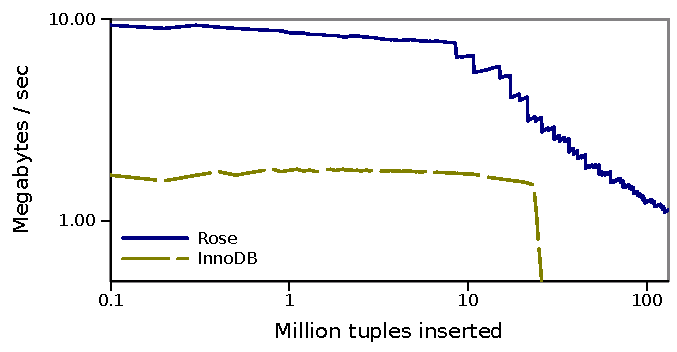
\epsfig{file=average-throughput.pdf, width=3.33in}
\caption{Insertion throughput (log-log, average over entire run).}
\label{fig:avg-thru}
\end{figure}
\begin{figure}
\centering
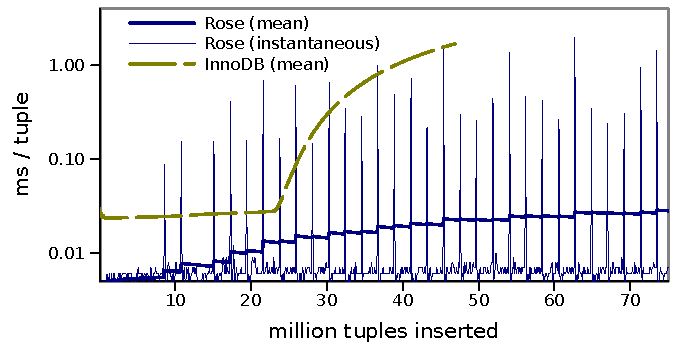
\epsfig{file=average-ms-tup.pdf, width=3.33in}
\caption{Tuple insertion time (log-log, average over entire run).}
\label{fig:avg-tup}
\end{figure}

As Figure~\ref{fig:avg-thru} shows, on an empty tree \rows provides
roughly 7.5 times more throughput than InnoDB.  As the tree size
increases, InnoDB's performance degrades rapidly.  After 35 million
tuple insertions, we terminated the InnoDB run, as \rows was providing
nearly 100 times more throughput.  We continued the \rows run until
the dataset was exhausted; at this point, it was providing
approximately $\frac{1}{10}$th its original throughput, and had a
target $R$ value of $7.1$.  Figure~\ref{fig:avg-tup} suggests that
InnoDB was not actually disk bound during our experiments; its
worst-case average tuple insertion time was approximately $3.4 ms$;
well below the drive's average access time.  Therefore, we believe
that the operating system's page cache was insulating InnoDB from disk
bottlenecks\footnote{In the process of running our experiments, we
  found that while \rows correctly handles 64-bit file offsets, and
  runs on 64-bit platforms, it crashes when given more than 2GB of
  RAM.}.  This problem with our experimental setup should work in InnoDB's favor.
\begin{figure}
\centering
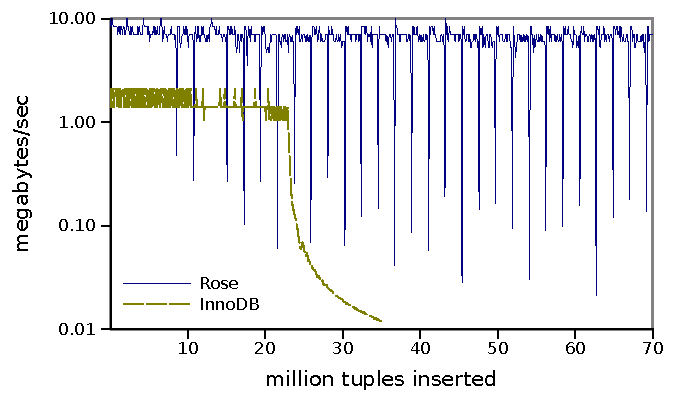
\epsfig{file=instantaneous-throughput.pdf, width=3.33in}
\caption{Instantaneous insertion throughput (average over 100,000 tuple windows).}
\label{fig:inst-thru}
\end{figure}

%\begin{figure}
%\centering
%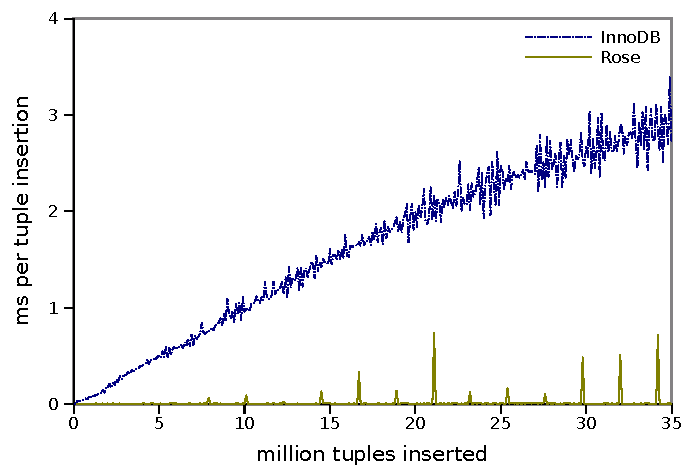
\epsfig{file=instantaneous-ms-tup.pdf, width=3.33in}
%\caption{Instantaneous tuple insertion time (average over 100,000 tuple windows).}
%\end{figure}

\subsection{Comparison with analytical model}

\rows outperforms B-Tree based solutions, as expected.  However, the
prior section says little about the overall quality of our prototype
implementation.  In this section, we measure update latency, compare
our implementation's performance with our simplified analytical model,
and discuss the effectiveness of \rowss compression mechanisms.

Figure~\ref{fig:inst-thru} reports \rowss replication throughput
averaged over windows of 100,000 tuple insertions.  The large downward
spikes occur periodically throughout our experimental run, though the
figure is truncated to only show the first 10 million inserts.  They
occur because \rows does not perform admission control, and updates
entire tree components atomically, rather than incrementally.
%  First, $C0$ accepts insertions at a much
%greater rate than $C1$ or $C2$ can accept them.  Over 100,000 tuples
%fit in memory, so multiple samples are taken before each new $C0$
%component blocks on the disk bound mergers.  Second, \rows merges
%entire trees at once, occasionally blocking smaller components
%for long periods of time while larger components complete a merge
%step.  Both of these problems could be masked by rate limiting the
%updates presented to \rows.
A better implementation would perform
incremental tree merges instead of merging entire components at once.

%This paper has mentioned a number of limitations in our prototype
%implementation.
Figure~\ref{fig:4R} seeks to quantify the overall performance
impact of our prototype's
limitations.  This figure uses our simplistic analytical model
to bound \rowss ideal disk throughput using \rowss
reported value of $R$.  According to our
model, we should expect an ideal, uncompressed version of \rows to
perform about twice as fast as our prototype performed during our experiments.  During our tests, \rows
maintains a compression ratio of two.  Therefore, our model suggests
that the prototype is running at $25\%$ of its ideal speed.

%% A number of factors contribute to the discrepancy between our model
%% and our prototype's performance.  First, the prototype's
%% whole-tree-at-a-time approach to merging forces us to make extremely
%% coarse and infrequent runtime adjustments to the ratios between tree
%% components.  This prevents \rows from reliably keeping the ratios near
%% the current target value for $R$.  Second, \rows currently
%% synchronously forces tree components to disk.  Given our large buffer
%% pool, a significant fraction of each new tree component is in the
%% buffer pool or operating system cache when the merge thread forces it
%% to disk.  This prevents \rows from overlapping I/O with computation.
%% Finally, our analytical model neglects some minor sources of storage
%% overhead.

%One other factor significantly limits our prototype's performance.
This is partially due to poor memory utilization.  Atomically
replacing $C0$ doubles \rows peak memory requirements, halving the
effective size of $C0$.  The balanced tree that we use seems to suffer
from memory fragmentation and again doubles $C0$'s memory
requirements.  Therefore, in our tests, the prototype was wasting
approximately $750MB$ of the $1GB$ we allocated to $C0$.

Finally, note that the analytical model's predicted throughput
increases with \rowss compression ratio.  Sophisticated, high-speed
compression routines achieve 4-32x compression ratios on TPC-H data,
while \rowss simplistic compression routines provide approximately 2x
compression.  Given ample processing power, these algorithms should
improve \rowss throughput by four to sixteen times.  XXX check cited ratios

%% Our performance figures show that \rows significantly outperforms a
%% popular, production quality B-Tree implementation.  Our experiments
%% reveal a number of deficiencies in our prototype implementation,
%% suggesting that further implementation efforts would improve its
%% performance significantly.  Finally, though our prototype could be
%% improved, it already performs at roughly $\frac{1}{4}$th of its ideal
%% throughput.  Our analytical models suggest that it will significantly
%% outperform any B-Tree implementation when applied to appropriate
%% update workloads.

\begin{figure}
\centering
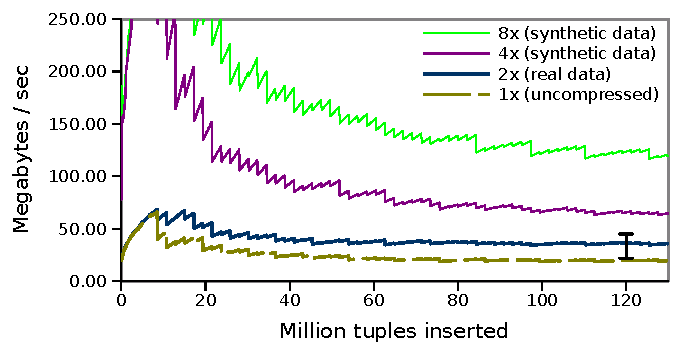
\epsfig{file=4R-throughput.pdf, width=3.33in}
\caption{The \rows prototype's effective bandwidth utilization.  Given
  infinite CPU time and a perfect implementation, our simplified model predicts $4R * throughput = sequential~disk~bandwidth *
  compression~ratio$.  (Our experimental setup never updates tuples in
  place)}
\label{fig:4R}
\end{figure}

\section{Related Work}

\subsection{LSM-Trees}

The original LSM-Tree work\cite{lsm} provides a more detailed
analytical model than the one presented above.  It focuses on update
intensive OLTP (TPC-A) workloads, and hardware provisioning for steady
state workloads.

Later work proposes the reuse of existing B-Tree implementations as
the underlying storage mechanism for LSM-Trees\cite{cidrPartitionedBTree}.  Many
standard B-Tree optimizations (such as prefix compression and bulk insertion)
would benefit LSM-Tree implementations.  \rows uses a custom tree
implementation so that it can take advantage of compression.
Compression algorithms used in B-Tree implementations must provide for
efficient, in place updates of tree nodes.  The bulk-load update of
\rows updates imposes fewer constraints upon our compression
algorithms.

Recent work on optimizing B-Trees for write intensive updates dynamically
relocates regions of B-Trees during
writes~\cite{bTreeHighUpdateRates}.  This reduces index fragmentation,
but still relies upon random I/O in the worst case.  In contrast,
LSM-Trees never use disk-seeks to service write requests, and produce
perfectly laid out B-Trees.

The problem of {\em Online B-Tree merging} is closely related to
LSM-Trees' merge process.  B-Tree merging addresses situations where
the contents of a single table index have been split across two
physical B-Trees that now need to be reconciled.  This situation
arises, for example, during rebalancing of partitions within a cluster
of database machines.

One particularly interesting approach lazily piggybacks merge
operations on top of tree access requests.  Upon servicing an index
probe or range scan, the system must read leaf nodes from both B-Trees.
Rather than simply evicting the pages from cache, lazy merging merges
the portion of the tree that has already been brought into
memory~\cite{onlineMerging}.

The original LSM-Tree paper proposes a mechanism that provides delayed
LSM-Tree index scans with no additional I/O.  The idea is to wait for
the merge thread to make a pass over the index, and to supply the
pages it produces to the index scan before evicting them from the
buffer pool.
By combining this idea with lazy merging, an LSM-Tree could service
range scans immediately without significantly increasing the amount of
I/O performed by the system.

\subsection{Row-based database compression}

Row-oriented database compression techniques compress each tuple
individually, and (in some cases) ignore similarities between adjacent
data items.  One such approach (for low cardinality data) builds a
table-wide mapping between short identifier codes and longer string
values. The mapping table is stored in memory for convenient
compression and decompression.  Other approaches include NULL
suppression, which stores runs of NULL values as a single count, and
leading zero suppression which stores integers in a variable length
format that suppresses leading zeros.  Row-based schemes typically
allow for easy decompression of individual tuples.  Therefore, they
generally store the offset of each tuple explicitly at the head of
each page.

Another approach is to compress page data using a generic compression
algorithm, such as gzip.  The primary drawback to this approach is
that the size of the compressed page is not known until after
compression.  Also, general purpose compression techniques typically
do not provide random access within pages and are often more processor
intensive than specialized database compression
techniques~\cite{rowImplementationPerf}.

\subsection{Column-oriented database compression}

Column-based compression is based on the observation that sorted
columns of data are often easier to compress than sorted tuples.  Each
column contains a single data type, and sorting decreases the
cardinality and range of data stored on each page.  This increases the
effectiveness of simple, special purpose, compression schemes.

PFOR (patched frame of reference) was introduced as an extension to
the MonetDB\cite{pfor} column-oriented database, along with two other
formats (PFOR-delta, which is similar to PFOR, but stores values as
deltas, and PDICT, which encodes columns as keys and a dictionary that
maps to the original values).  We plan to add both these formats to
\rows in the future.  We chose to implement RLE and PFOR because they
are amenable to superscalar optimization, and compression is \rowss
primary CPU bottleneck.  Like MonetDB, each \rows table is supported
by custom-generated code.

C-Store, another column oriented database, has relational operators
that have been optimized to work directly on compressed
data\cite{compExec}.  For example, when joining two run length encoded
columns, it is unnecessary to explicitly represent each row during the
join.  This optimization would be particularly useful in \rows, as its
merge processes perform repeated joins over compressed data.  Our
prototype does not make use of these optimizations, though they would
likely improve performance for CPU-bound workloads.

A recent paper provides a survey of database compression
techniques and characterizes the interaction between compression
algorithms, processing power and memory bus bandwidth.  To the extent
that multiple columns from the same tuple are stored within the same
page, all formats within their classification scheme group information
from the same tuple together~\cite{bitsForChronos}.

\rows, which does not split tuples across pages, takes a different
approach, and stores each column separately within a page.  Our column
oriented page layouts incur different types of per-page overhead, and
have fundamentally different processor
cache behaviors and instruction-level parallelism properties than the
schemes they consider.

In addition to supporting compression, column databases typically
optimize for queries that project away columns during processing.
They do this by precomputing the projection and potentially resorting
and recompressing the data.  This reduces the amount of data on the
disk and the amount of I/O performed by the query.  In a
column store, such optimizations happen off-line, leading to
high-latency inserts.  \rows can support such optimizations by
producing multiple LSM-Trees for a single table.

Unlike read-optimized column-oriented databases, \rows is optimized
for write throughput, and provides low-latency, in-place updates.
This property does not come without cost; compared to a column
store, \rows must merge replicated data more often, achieves lower
compression ratios, and performs index lookups that are roughly twice
as expensive as a B-Tree lookup.

\subsection{Snapshot consistency}

\rows relies upon the correctness of the master database's concurrency
control algorithms to provide snapshot consistency to queries.  \rows
is compatible with the two most popular approaches to concurrency
control in OLTP environments: two-phase locking and timestamps
(multiversion concurrency control).

\rows only provides read-only queries.  Therefore, its concurrency
control algorithms need only address read-write conflicts.
Well-understood techniques protect against read-write conflicts
without causing requests to block, deadlock or
livelock~\cite{concurrencyControl}.

\subsection{Log shipping}

Log shipping mechanisms are largely outside the scope of this paper;
any protocol that provides \rows replicas with up-to-date, intact
copies of the replication log will do.  Depending on the desired level
of durability, a commit protocol could be used to ensure that the
\rows replica receives updates before the master commits.  Because
\rows is already bound by sequential I/O throughput, and because the
replication log might not be appropriate for database recovery, large
deployments would probably opt to store recovery and logs on machines
that are not used for replication.

\section{Conclusion}

Compressed LSM trees are practical on modern hardware.  As CPU
resources increase, improved compression ratios will improve \rowss
throughput by decreasing its sequential I/O requirements.  In addition
to applying compression to LSM-Trees, we presented a new approach to
database replication that leverages the strengths of LSM-Trees
by avoiding index probing during updates.  We also introduced the idea of using
snapshot consistency to provide concurrency control for LSM-Trees.
%% Our prototype's LSM-Tree recovery mechanism is extremely
%% straightforward, and makes use of a simple latching mechanism to
%% maintain our LSM-Trees' consistency.  It can easily be extended to
%% more sophisticated LSM-Tree implementations that perform incremental
%% tree merging.

Our implementation is a first cut at a working version of \rows.
We have characterized the performance of our prototype, and
bounded the performance gain we can expect to achieve via further
optimizations.  By avoiding disk seeks for all operations except
random index probes, uncompressed LSM-Trees can outperform
B-Tree based indices by at least 2 orders of magnitude.  With real-world
database compression ratios ranging from 5-20x, we expect \rows
database replicas to outperform B-Tree based database replicas by an
additional factor of ten.

We implemented \rows to address scalability issues faced by large
scale database installations.  \rows addresses seek-limited
applications that require real-time analytical and decision
support queries over extremely large, frequently updated data sets.
As automated financial transactions and other real-time database
applications become more popular,
applications with these requirements are becoming increasingly common.

XXX fix conclusion sentence.

\bibliographystyle{abbrv}
\bibliography{rose}  % sigproc.bib is the name of the Bibliography in this case
% You must have a proper ".bib" file
%  and remember to run:
% latex bibtex latex latex
% to resolve all references
%
% ACM needs 'a single self-contained file'!
%
\balancecolumns % GM July 2000
% That's all folks!
\end{document}
